\documentclass[letterpaper,english,11pt]{article}
\usepackage{%
	amsfonts,%
	amsmath,%	
	amssymb,%
	amsthm,%
	babel,%
	bbm,%
	%biblatex,%
	caption,%
	centernot,%
	color,%
	enumerate,%
	%enumitem,%
	epsfig,%
	epstopdf,%
	etex,%
	fancybox,%
	framed,%
	fullpage,%
	%geometry,%
	graphicx,%
	hyperref,%
	latexsym,%
	mathptmx,%
	mathtools,%
	multicol,%
	pgf,%
	pgfplots,%
	pgfplotstable,%
	pgfpages,%
	proof,%
	psfrag,%
	%subfigure,%	
	tikz,%
	times,%
	ulem,%
	url,%
	xcolor,%
	mathpazo
}

\definecolor{shadecolor}{gray}{.95}%{rgb}{1,0,0}
\usepackage[margin=1in,top=0.75in]{geometry}
\usepackage[mathscr]{eucal}
\usepgflibrary{shapes}
\usepgfplotslibrary{fillbetween}
\usetikzlibrary{%
  arrows,%
  backgrounds,%
  chains,%
  decorations.pathmorphing,% /pgf/decoration/random steps | erste Graphik
  decorations.text,% 
  matrix,%
  positioning,% wg. " of "
  fit,%
  patterns,%
  petri,%
  plotmarks,%
  scopes,%
  shadows,%
  shapes.misc,% wg. rounded rectangle
  shapes.arrows,%
  shapes.callouts,%
  shapes%
}

%\pgfplotsset{compat=newest} %<------ Here
\pgfplotsset{compat=1.11} %<------ Or use this one

\theoremstyle{plain}
\newtheorem{thm}{Theorem}[section]
\newtheorem{lem}[thm]{Lemma}
\newtheorem{prop}[thm]{Proposition}
\newtheorem{cor}[thm]{Corollary}
\newtheorem{clm}[thm]{Claim}

\theoremstyle{definition}
\newtheorem{axiom}[thm]{Axiom}
\newtheorem{defn}[thm]{Definition}
\newtheorem{conj}[thm]{Conjecture}
\newtheorem{exmp}[thm]{Example}
\newtheorem{exerc}[thm]{Exercise}
\newtheorem{assum}[thm]{Assumptions}

\theoremstyle{remark}
\newtheorem{rem}[thm]{Remark}
\newtheorem{note}[thm]{Note}

\newcommand{\Cov}{\operatorname{Cov}}
%\newcommand{\det}{\operatorname{det}}
\newcommand{\Real}{\mathbb{R}}
\newcommand{\tr}{\operatorname{tr}}
%\newcommand{\Var}{\operatorname{Var}}

\DeclareMathOperator{\sign}{sign}
%\renewcommand{\proof}[1]{\begin{proof}#1\end{proof}}
\newcommand{\EQ}[1]{\begin{equation*}#1\end{equation*}}
\newcommand{\EQN}[1]{\begin{equation}#1\end{equation}}
\newcommand{\eq}[1]{\begin{align*}#1\end{align*}}
\newcommand{\meq}[2]{\begin{xalignat*}{#1}#2\end{xalignat*}}
\newcommand{\norm}[1]{\left\lVert#1\right\rVert}
\newcommand{\abs}[1]{\left\lvert#1\right\rvert}
\newcommand{\expect}[1]{\mathbb{E}\left[{#1}\right]}
\newcommand{\prob}[1]{\mathbb{P}\left[{#1}\right]}
\newcommand{\given}{\; \big\vert \;} 
\newcommand{\set}[1]{\left\{#1\right\}} 
\newcommand{\indicator}[1]{\mathbb{1}_{\set{#1}}} 
\newcommand{\inner}[1]{\left\langle#1\right\rangle}
\newcommand{\red}[1]{\textcolor{red}{#1}} 
\newcommand{\E}[1]{\mathbb{E}\left[#1\right]}
\newcommand{\Var}[1]{\operatorname{Var}\left[#1\right]}

\newcommand{\D}{\mathbb{D}}
%\newcommand{\E}{\mathbb{E}}
\newcommand{\N}{\mathbb{N}}
\renewcommand{\P}{\mathbb{P}}
\newcommand{\Q}{\mathbb{Q}}
\newcommand{\R}{\mathbb{R}}
\newcommand{\Z}{\mathbb{Z}}

\newcommand{\bU}{\mathbf{1}}
\newcommand{\bx}{\mathbf{x}}

\newcommand{\cB}{\mathcal{B}}
\newcommand{\cC}{\mathcal{C}}
\newcommand{\cD}{\mathcal{D}}
\newcommand{\cF}{\mathcal{F}}
\newcommand{\cG}{\mathcal{G}}
\newcommand{\cH}{\mathcal{H}}
\newcommand{\cO}{\mathcal{O}}
\newcommand{\cT}{\mathcal{T}}
\newcommand{\cX}{\mathcal{X}}
\newcommand{\cY}{\mathcal{Y}}

\newcommand{\sA}{\mathscr{A}}
\newcommand{\sB}{\mathscr{B}}
\newcommand{\sC}{\mathscr{C}}
\newcommand{\sD}{\mathscr{D}}
\newcommand{\sE}{\mathscr{E}}
\newcommand{\sF}{\mathscr{F}}
\newcommand{\sG}{\mathscr{G}}
\newcommand{\sH}{\mathscr{H}}
\newcommand{\sL}{\mathscr{L}}
\newcommand{\dO}{\mathscr{O}}
\newcommand{\sS}{\mathscr{S}}
\newcommand{\sT}{\mathscr{T}}
\newcommand{\sX}{\mathscr{X}}
\newcommand{\sY}{\mathscr{Y}}
\newcommand{\sZ}{\mathscr{Z}}

% Debug
\newcommand{\todo}[1]{\begin{color}{blue}{{\bf~[TODO:~#1]}}\end{color}}

% a few handy macros

\renewcommand{\le}{\leqslant}
\renewcommand{\ge}{\geqslant}
\newcommand\matlab{{\sc matlab}}
\newcommand{\goto}{\rightarrow}
\newcommand{\bigo}{{\mathcal O}}
%\newcommand{\half}{\frac{1}{2}}
%\newcommand\implies{\quad\Longrightarrow\quad}
\newcommand\reals{{{\rm l} \kern -.15em {\rm R} }}
\newcommand\complex{{\raisebox{.043ex}{\rule{0.07em}{1.56ex}} \hskip -.35em {\rm C}}}


% macros for matrices/vectors:

% matrix environment for vectors or matrices where elements are centered
\newenvironment{mat}{\left[\begin{array}{ccccccccccccccc}}{\end{array}\right]}
\newcommand\bcm{\begin{mat}}
\newcommand\ecm{\end{mat}}

% matrix environment for vectors or matrices where elements are right justifvied
\newenvironment{rmat}{\left[\begin{array}{rrrrrrrrrrrrr}}{\end{array}\right]}
\newcommand\brm{\begin{rmat}}
\newcommand\erm{\end{rmat}}

% for left brace and a set of choices
%\newenvironment{choices}{\left\{ \begin{array}{ll}}{\end{array}\right.}
\newcommand\when{&\text{if~}}
\newcommand\otherwise{&\text{otherwise}}
% sample usage:
%  \delta_{ij} = \begin{choices} 1 \when i=j, \\ 0 \otherwise \end{choices}


% for labeling and referencing equations:
\newcommand{\eql}{\begin{equation}\label}
\newcommand{\eqn}[1]{(\ref{#1})}
% can then do
%  \eql{eqnlabel}
%  ...
%  \end{equation}
% and refer to it as equation \eqn{eqnlabel}.  


% some useful macros for finite difference methods:
\newcommand\unp{U^{n+1}}
\newcommand\unm{U^{n-1}}

% for chemical reactions:
\newcommand{\react}[1]{\stackrel{K_{#1}}{\rightarrow}}
\newcommand{\reactb}[2]{\stackrel{K_{#1}}{~\stackrel{\rightleftharpoons}
   {\scriptstyle K_{#2}}}~}


\makeatletter
\def\th@plain{%
  \thm@notefont{}% same as heading font
  \itshape % body font
}
\def\th@definition{%
  \thm@notefont{}% same as heading font
  \normalfont % body font
}
\makeatother
\date{}

\usepackage{algorithm2e}
\usepackage{bm}
%opening
\title{Lecture-27: Random K-SAT and Combinatorial Optimization}
\author{Author: V. Arvind Rameshwar}

\begin{document}
\maketitle
\section{The Satisfiability (SAT) Problem}

The SAT problem (sometimes called the Boolean SAT problem) is a classical question that seeks to check if a given Boolean formula indeed has a satisfying assignment to its variables. SAT has quite some historical significance attached to it, owing to the fact that it was the first problem to be proved \textit{NP-complete}, in the seminal work of Cook in 1971 (and independently, by Leonid Levin in 1973), leading to a variety of other problems being proved as NP-complete, by way of polynomial-time-reductions to SAT. In what follows, we shall clearly define the SAT decision problem, and the K-SAT problem, in particular, followed by a discussion on the factor-graph representation of K-SAT.\\

Let $x_1,x_2,\ldots,x_N\in \{0,1\}$ be $N$ Boolean variables. Further, let $S_1,S_2,\ldots,S_M\subset [N]$ be $M$ arbitrary subsets of the set of integers from $1$ to $N$. 
\begin{defn}(Literal)
A literal is either a variable or its negation; in particular, the $j^{\text{th}}$ literal, $w_j$, is either $x_j$ or $\overline{x_j}$, for $j\in [N]$.
\end{defn}
\begin{defn}(Clause)
A clause with neighbourhood $S$ is a disjunction (OR) of literals in $S$; in particular, the $m^{\text{th}}$ clause, $C_m$, for $m\in [1:M]$, is given by:
\begin{equation*}
    C_m = \bigvee_{j\in S_m} w_j,
\end{equation*}
for given literals $\{w_1,\ldots,w_N\}$ and $S_m$ as defined previously. 
\end{defn}
\begin{defn}(CNF Formula)
 Given $N$ Boolean variables $x_1,\ldots,x_N$, and subsets $S_1,\ldots,S_M$, a Boolean function $F$ is said to be in \textit{Conjunctive Normal Form} (or $F$ is a CNF formula) if it has the following structure:
\begin{equation*}
    F=C_1\wedge C_2\wedge \ldots \wedge C_M,
\end{equation*}
for clauses $C_1,\ldots,C_M$ with neighbourhoods $S_1,\ldots,S_M$ respectively.
\end{defn}
\begin{rem}
A CNF formula is a conjunction of clauses, where each clause is a disjunction of literals.
\end{rem}
With these definitions in place, we can now formally introduce the SAT problem:
\begin{defn}(SAT)
Given a Boolean function F over $N$ variables and $M$ clauses, in CNF form, the SAT decision problem is to determine if there exists a \textit{satisfying assignment}, i.e., an assignment vector, ${\mathbf{A}}$, of values to $\{x_1,\ldots,x_N\}$ such that $F({\mathbf{A}}) = 1$.

If such an assignment exists, the formula $F$ is said to be SAT. Otherwise, it is said to be UNSAT.
\end{defn}
Several special cases of the SAT formulation can be constructed---of interest to us, however, is the K-SAT problem, defined as follows:

\begin{defn}(K-SAT)
The K-SAT decision problem is the SAT decision problem, where the CNF formula, $F$, is such that $|S_1|=|S_2|=\ldots=|S_M|=K$.
\end{defn}

\begin{shaded*}
\begin{exmp}
As an example, we consider the 3-SAT problem:
\begin{equation*}
    F = (x_1\vee x_2\vee x_3)\wedge(\overline{x_1}\vee \overline{x_2}\vee x_3)\wedge(\overline{x_1}\vee x_2\vee \overline{x_3}).
\end{equation*}
It is easy to verify that the 3-SAT instance, $F$ above, is SAT, with $\mathbf{A} = \{1,1,1\}$.
\end{exmp}
\end{shaded*}
\begin{rem}
We shall henceforth use the indices $a,b,c,\ldots$ to denote clauses, and $i,j,k,\ldots$ to denote the indices of literals. Also, we shall use the notation $\partial a$ to denote the set of literals contained in clause $a$, and $\partial i$ to denote the set of clauses that literal $w_i$ is present in.
\end{rem}
\subsection{Factor Graph Representation}
Associated with a K-SAT formula, $F$, is a natural bipartite factor graph, $\mathscr{G}_{F} = ((V,\mathscr{F}),\mathscr{E})$, where $V=[N]$ and $\mathscr{F}=\{C_1,\ldots,C_M\}$. An edge $(i,a)\in \mathscr{E}$ if $w_i\in \partial a$. For an edge $e=(i,a)$, its weight $J_{ia}$ is given by:
\begin{equation*}
    J_{ia} = 
    \begin{cases}
    +1,\quad \text{if } x_i\in \partial a,\\
    -1,\quad \text{if } \overline{x_i}\in \partial a,\\
    \end{cases}
\end{equation*}

For $x_i\in \{0,1\}$, we define $s_i=(-1)^{x_i}\in \{-1,+1\}$.\\

Given such a factor graph, it is easy to define a product form function,
\begin{equation*}
    \beta_{F}(\mathbf{s}) = \prod_{a=1}^{M}\left(1-\frac{1}{2^K}\left(\prod_{i\colon x_i\in \partial a}\left(1-J_{ia}s_i\right)\right)\right).
\end{equation*}
It is easy to see that for any vector $\mathbf{s}\in \{-1,+1\}^{N}$, $\beta_{F}(\mathbf{s}) \in \{0,1\}$, and is equal to $1$ if and only if $\mathbf{s}$ is a satisfying assignment for $F$.\\

Further, the marginal of $\beta_{F}(\mathbf{s})$ onto $s_i=+1$, for $i\in [N]$, gives us the number of SAT assignments with $x_i = 0$. Hence, applying standard Belief-Propagation algorithms when $\mathscr{G}_{F}$ is a tree, will give us the number of such SAT assignments with one variable fixed. It is to be noted, however, that this is not a procedure to \textit{solve} the K-SAT instance.

\section{Algorithms for K-SAT}
\subsection{K=1}
For this restricted setting, it is simple to devise a linear-time algorithm, to check if a Boolean formula, $F$, is SAT: $F$ is SAT if and only if $F$ does not contain both $x_i$ and $\overline{x_i}$, for some $i\in [N]$.

\begin{shaded*}
\begin{exmp}
$F = x_1\wedge x_2\wedge x_3\wedge \overline{x_1}$ is UNSAT.
\end{exmp}
\end{shaded*}
\subsection{K=2}

\begin{shaded*}
\begin{exmp}
Before we describe an algorithm for 2-SAT, we shall look at an example: $F=(x_1\vee \overline{x_2})\wedge(x_2\vee \overline{x_3})\wedge(x_3\vee \overline{x_1})$. We first pick $x_1=0$. This forces $x_2$ to be $0$, which in turn, forces $x_3$ to be $0$. Thus, $\mathbf{A} = \{0,0,0\}$ is a satisfying assignment, for $F$.
\end{exmp}
\end{shaded*}

We shall now extend the procedure detailed out in the example above, to an algorithm called \textbf{UCP} (for Unit Clause Propagation). The algorithm proceeds by fixing $x_1$ to be $0$, and then iteratively reduces $F$ to $F_1$, by removing clauses containing $\overline{x_1}$, and force-satisfying clauses containing $x_1$. If $F_1$ contains $x_j\wedge \overline{x_j}$, for some $j\in [N]$, then the value of $x_1$ is changed to $1$. Otherwise, \textbf{UCP} repeats the procedure on $F=F_1$, by now fixing the variable with smallest index, remaining, to be $0$.

The only way \textbf{UCP} can fail to produce a satisfying assignment, is when $x_j$, for some $j\in [N]$, can not be $0$ or $1$, in which case, \textbf{UCP} declares that $F$ is UNSAT.

It is easy to check that the complexity of \textbf{UCP} is $O(N)$, since each variable, $x_i$, $i\in [N]$, is considered at most twice.

\subsection{K=3}
Since 3-SAT is NP-hard, we can only resort to probabilistic algorithms for this case. The most popular algorithm is probably the one by Sch\"oning, given below.

\begin{figure}[h]
\centering
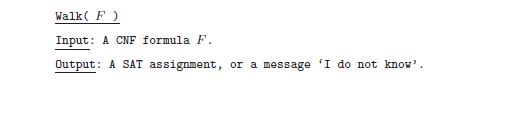
\includegraphics[scale=1.4]{./Figures/Schoning1.JPG}
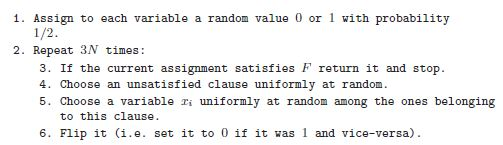
\includegraphics[scale=1.3]{./Figures/Schoning2.JPG}
\caption{The algorithm, Walk($F$), by Sch\"oning (Source: M\'ezard and Montanari).}
\end{figure}

\begin{prop}
Let $p_S(F)$ be the probability that Walk($F$) returns $1$, when $F$ is SAT. Then,
\begin{equation*}
    p_S(F)\geq \frac{2}{3}\left(\frac{K}{2(K-1)}\right)^{N}.
\end{equation*}
\end{prop}
\begin{proof}
Let $\mathbf{A}^{*}$ be a SAT assignment for $F$. Let $\mathbf{A}^{t}$ be the assignment produced by Walk($F$), after $t$ iterations.

Denote by $d^{t}:= d_H(\mathbf{A}^{*},\mathbf{A}^{t})$, the Hamming distance between $\mathbf{A}^{*}$ and $\mathbf{A}^{t}$. Clearly,
\begin{equation*}
    \mathbb{P}(d^0=d)={N\choose d}\frac{1}{2^N}.
\end{equation*}
For any unsatisfied clause, Step 5. reduces $d^{t}$ by 1, with probability at least $1/K$. This is because, the probability that the algorithm picks a variable to flip, that disagrees in its value with $\mathbf{A}^{*}$, is at least $1/K$.

Consider exactly one such ``candidate" variable per clause, and introduce an auxiliary variable, $\hat{d^{t}}$, that reduces by one each time such a candidate is chosen, and increases by one, otherwise.

We observe that:

\begin{equation*}
    \hat{d^{t}}\geq d^{t} \quad \text{and}\quad \mathbb{P}(\hat{d^{t}}=0)\leq \mathbb{P}({d^{t}}=0). 
\end{equation*}

Note that the sequence of random variables, $\{\hat{d^{t}}\}_{t\geq 0}$, forms a Markov Chain on the set of integers $[0:N]$. The probability of transition from state $i$ to $i+1$ is $1-1/K$, and the transition probability from $i$ to $i-1$ is $1/K$, for all states $i\in[1:N-1]$. Now, for some $t$,
\begin{align*}
    \mathbb{P}(\hat{d^{0}}=d,\hat{d^{t}}=0) &= \frac{1}{2^N}{N\choose d}{t\choose \frac{t-d}{2}}\left(1-\frac{1}{K}\right)^{\frac{t-d}{2}}\left(\frac{1}{K}\right)^{\frac{t+d}{2}}\\
    &\stackrel{.}{=}_{\small{N}} 2^{-N\left(1-\mathcal{H}\left(\frac{d}{N}\right)-\frac{t}{N}\mathcal{H}\left(\frac{t-d}{2t}\right)+\frac{t}{N}logK-\left(\frac{t-d}{2N}\right)log(K-1)\right)}\\
    &=: 2^{-N\psi(\theta,\delta)},
\end{align*}
where $\theta=\frac{t}{N}$ and $\delta = \frac{d}{N}$, and $\mathcal{H}(.)$ is the binary entropy function. The first equality follows from the fact that the $d$ variables that differ in value with $\mathbf{A}^{*}$, at $t=0$, are chosen uniformly at random from the $N$ possible choices.

We observe that for $\theta \in [0,3]=:I_{\theta}$ and $\delta \in [0,1]=:I_{\delta}$,
\begin{equation*}
    \min_{I_{\theta}, I_{\delta}}\psi(\theta,\delta) = \log \left(\frac{2(K-1)}{K}\right),
\end{equation*}
which completes the proof.
\end{proof}
\begin{rem}
One way to think about the result above, is that the \text{expected} number of runs of Walk($F$) that need to be performed, before reaching a satisfying assignment, is of the order of $(1.33)^{N}$, for $K=3$.
\end{rem}
\section{Random K-SAT Ensembles}

In the previous sub-section, we had a look at a probabilistic algorithm, Walk($F$), that could identify a satisfying assignment for $F$ (provided that it is indeed SAT), by doing better than brute-force-search. We are now interested in characterizing ``easy instances" of K-SAT problems, that are satisfiable with probability $1$, as $N\rightarrow \infty$.

To do so, we need to consider ensembles of SAT instances.

\begin{defn}(K-SAT ensemble)
The ensemble $\text{SAT}_N(K,M)$ is obtained by selecting $M$ clauses, $C_1,C_2,\ldots,C_M$, with $|S_1|=|S_2|=\ldots=|S_M|=K$, uniformly at random from the ${N\choose K}2^{K}$ possible clauses.
\end{defn}

Let $\alpha:=\frac{M}{N}$ and let $P_{N}(K,\alpha)$ denote the probability that a K-SAT instance drawn from $\text{SAT}_N(K,M)$ is satisfiable.

\subsection{Random 2-SAT}

With the definitions above in place, we introduce the following theorem by Chv\'atal and Reed (`92):

\begin{thm} (CR)\label{CR}
Consider the $\text{SAT}_N(K=2,M)$ ensemble. Then,
\begin{equation*}
    \lim_{N\rightarrow \infty} P_{N}(K=2,\alpha) = \begin{cases}
    1,\quad \text{if }\alpha<1,\\
    0,\quad \text{if }\alpha>1\\
    \end{cases}.
\end{equation*}

In other words, the ensemble exhibits a phase transition at $\alpha_c=1$.
\end{thm}

Before we proceed to prove this theorem, we require some additional machinery. Given a (random) $2$-SAT instance $F$, with $N$ variables and $M$ clauses, we associate with it, a directed graph, $D_{F}(\tilde{V},\tilde{\mathscr{E}})$, with
\begin{equation*}
    \tilde{V}=\{x_1,x_2,\ldots,x_N,\overline{x_1},\overline{x_2},\ldots,\overline{x_N}\},\quad\text{and}
\end{equation*}
\begin{equation*}
    \text{for }C_l=(w_{i_{1,l}},w_{i_{2,l}}),\quad (\overline{w_{i_{1,l}}},w_{i_{2,l}})\text{ and }(\overline{w_{i_{2,l}}},w_{i_{1,l}})\in \tilde{\mathscr{E}},
\end{equation*}
where $1\leq l\leq M$ and $1\leq i_{1,l},i_{2,l}\leq N$.\\

As an example, for $F=(x_1\vee \overline{x_2})\wedge(x_2\vee \overline{x_3})\wedge(x_3\vee \overline{x_1})$, $D_F$ looks like the graph in Figure \ref{fig:graph}. 
\begin{figure}[h]
\centering
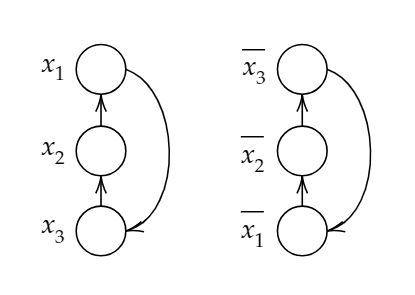
\includegraphics[scale=0.6]{./Figures/Directed_graph.JPG}
\caption{The directed graph, $D_F$, for the given formula $F$.}
\label{fig:graph}
\end{figure}
We now claim that the following lemma holds, for a given directed graph, $D_F$.
\begin{lem}
$F$ is UNSAT iff there exists $i\in [N]$ such that $D_F$ has a directed cycle containing both $x_i$ and $\overline{x_i}$.
\end{lem}
\begin{proof}
(``If" part):\\
Since there exists a path from $x_i$ to $\overline{x_i}$, setting $x_i$ to $1$ leads to a contradiction.\\
Similarly, since there exists a path from $\overline{x_i}$ to ${x_i}$, setting $x_i$ to $0$ leads to a contradiction.\\

(``Only if" part):\\
Since \textbf{UCP} yields correct results for $2$-SAT, we get that $F$ is UNSAT iff \textbf{UCP} fails. This happens only when there exists a variable, $x_j$, that cannot take the values $0$ or $1$. Retracing the arguments in the ``if" part backwards, we arrive at the result. 
\end{proof}

With the above lemma at hand, we can proceed with a proof of Theorem \ref{CR}.
\begin{proof}
(Of Theorem \ref{CR}):\\
We endeavour to prove only the first part, i.e., that $\lim_{N\rightarrow \infty}P_N(K=2,\alpha)=1$, if $\alpha<1$.
Given a $2$-SAT instance $F$, consider the corresponding $D_F$. We define a \textit{bicycle} of length $s$, to be a path $(u,w_1,w_2,\ldots,w_s,v)$, where $w_i,\text{ }i\in [N]$, are literals on $s$ \textit{distinct} variables. Further, $u,v\in\{w_1,\ldots,w_s,\overline{w_1},\ldots,\overline{w_s}\}$. Now, we make the following observation:
\begin{equation*}
    \{D_F\text{ has a directed cycle containing }x_i,\overline{x_i}\text{ for some }i\}\subset \{D_F\text{ has a bicycle}\},
\end{equation*}
and hence,
\begin{align*}
\mathbb{P}(F\text{ is UNSAT})&\leq \mathbb{P}(D_F\text{ has a bicycle})\\
&=\sum_{s=2}^{N}{N\choose s}2^{s}(2s)^{2}{M\choose s+1}\left(\frac{1}{4{N\choose 2}}\right)^{s+1}\\
&\leq \sum_{s=2}^{N}N^{s}2^{s}(2s)^{2}M^{s+1}\left(\frac{1}{4{N\choose 2}}\right)^{s+1}\\
&=\frac{M}{{N\choose 2}}\sum_{s=2}^{N}\left(\frac{M}{N-1}\right)^{s},
\end{align*}
which in the limit as $N$ goes to infinity, goes to $0$, so long as $\frac{M}{N-1}<1$, or $\alpha<1$.
\end{proof}
\begin{rem}
Note that the above proof only provides a \textit{lower bound} on $\alpha_c$. In order to arrive at the matching upper bound, we need some further techniques, which we shall not develop in this lecture.
\end{rem}
\section{Summary}
In this lecture, we have considered the K-SAT formulation in detail, first in the setting where the formula, $F$, is given, and later, when $F$ is drawn from the ensemble, $\text{SAT}_N(K,M)$. In the former case, we analyzed deterministic poly-time algorithms for $K=1,2$ and also provided a probabilistic algorithm, Walk($F$), for $K=3$. In the latter case, we identified the existence of a phase transition for $K=2$, with the threshold being $\alpha_c=(M/N)_c=1$.

\begin{thebibliography}{7}
\nocite{*}
\bibitem{r1}
V. Chvatal and B. Reed. 1992. ``Mick gets some (the odds are on his side) (satisfiability)". In Proceedings of the 33rd Annual Symposium on Foundations of Computer Science (SFCS '92). IEEE Computer Society, Washington, DC, USA, 620-627. DOI: https://doi.org/10.1109/SFCS.1992.267789

\bibitem{r2}
Uwe Schöning. 1999. ``A Probabilistic Algorithm for k-SAT and Constraint Satisfaction Problems". In Proceedings of the 40th Annual Symposium on Foundations of Computer Science (FOCS '99). IEEE Computer Society, Washington, DC, USA, 410-.

\bibitem{r3}
Marc Mezard and Andrea Montanari. 
``Information, Physics, and Computation".
Oxford University Press, Inc., New York, NY, USA,2009. 
\end{thebibliography}
\end{document}